\documentclass[tikz]{standalone}

\begin{document}
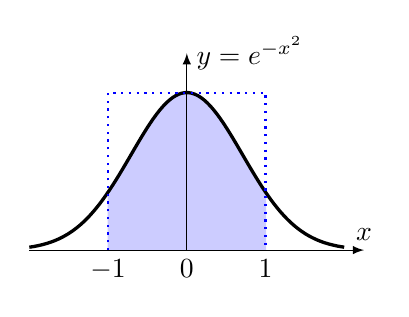
\begin{tikzpicture}[yscale=2]
  \filldraw[fill=blue!20, domain=-1:1, samples=100, color=blue!20] (-1,0)--plot( {\x}, {exp(-(\x)^2}) -- (1,0) -- cycle;
  \draw[-latex] (-2,0)--(2.25,0) node[above] {\(x\)};
  \draw[-latex] (0,0)--(0,1.25) node[right] {\(y=e^{-x^2}\)};
  \draw[very thick, domain=-2:2, variable=\z, samples=100]
  plot( {\z}, {exp(-(\z)^2});
  \node[below] at (0,0) {\(0\)};
  \node[below] at (-1,0) {\(-1\)};
  \node[below] at (1,0) {\(1\)};
  \draw[dotted, color=blue, thick] (-1,0)--(-1,1)--(1,1)--(1,0);
\end{tikzpicture}
\end{document}
